\section{The Least Absolute Deviations Method}

As we have seen previously, the core of the Ordinary Least Squares method (OLS) is finding the model vector -- $\hat{w}$ -- that minimizes the \emph{squared error} -- also known as the \emph{quadratic loss} -- between the prediction we are able to make -- i.e. $\hat{Y} = X\hat{w}$ -- and the true values of Y that we know from the training set. 

As we have seen before, we can express all this in a very compact form when using a matrix notation. So,  the errors we make when fitting the traning data can be stored in the $\epsilon$ is the vector, given by

\begin{equation}
\epsilon = Y - \hat{Y} = Y - X \hat{w} 
\end{equation}
the quadratic loss is given by:
\begin{equation}
\epsilon^T \epsilon = (Y - X \hat{w})^{T}(Y - X \hat{w})
\end{equation}
We wish to find the best $\hat{w}$, i.e. the one that minimize the squared error, and this is found by finding the zero of the first derivative of $\epsilon$ in order to $\hat{w}$:
\begin{equation}
\frac{\partial \epsilon^T \epsilon}{\partial \hat{w}} = 0
\end{equation}
The fact that we (arbitrarily?) chose to use the squared error to measure the fit (or lack of fit) of the model to the data is very convinient because it allows us to allows us to symbolically compute the derivative of $\epsilon$ in relation to $\hat{w}$, and from there find the zeros by simple algebraic manipulation. We can that obtain a closed form solution for $\hat{w}$, which is given (as we have seen) by:
\begin{equation}
\hat{w} = (X^T X)^{-1} X^T Y
\end{equation}
The mathematical convience provided by the choice of the squared loss comes, however, at a cost: when trying to estimation the model parameter (i.e. $\hat{w}$) we will be exposed to increased sensitiveness to the presence of outliers in the traning set. What this means even if most of the point in the X / Y dataset do follow a linear trend (meaning that they would be accurately captured by our linear model), the presence of a few outliers points (that don't follow that linear trend) will significantly impact the estimation of $\hat{w}$. So, we may end with significantly different $\hat{w}$ just depending on the inclusion or exclusion of a very small fraction of points. 

To illustrate this lets consider that we estimate parameters of a logistic regression in two situations. In the first situation we generate data by using the following equation:
\begin{equation}
y_i = 1 + 2 x_i + \mathcal{N}_i(0,1)
\end{equation}
which corresponds to having a linear relation 
\begin{equation}
Y = Xw + \mathcal{N}(0,1)
\label{eq.linear_relation_for_simulation}
\end{equation}
with:
\begin{equation}
w = 
\begin{bmatrix}
w_0\\
w_1\\
\end{bmatrix}
= 
\begin{bmatrix}
1\\
2\\
\end{bmatrix}
\end{equation}
Figures \ref{fig.ols_estimates_no_outliers} shows the distribution of values obtained while estimating $w_0$ and $w_1$ for 10000 runs. In each of those runs we we generate the 500 (X, Y) points data using Equation \ref{eq.linear_relation_for_simulation} and we try to estimate $w_0$ and $w_1$ using Ordinary Least Squares (OLS).

\begin{figure}
\centering
\begin{minipage}{.5\textwidth}
  \centering
  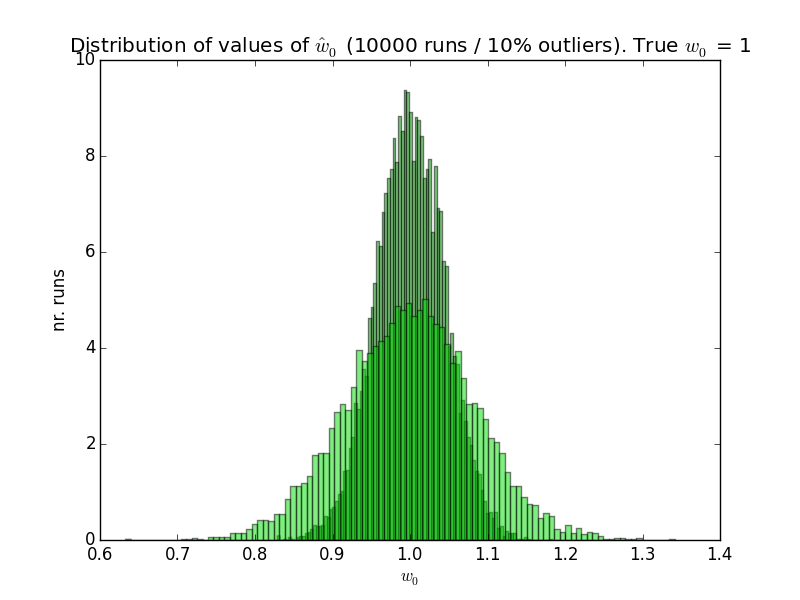
\includegraphics[width=1.0\linewidth]{chapter_lad/ols_w0_with_and_without_outliers.png}
\end{minipage}%
\begin{minipage}{.5\textwidth}
  \centering
  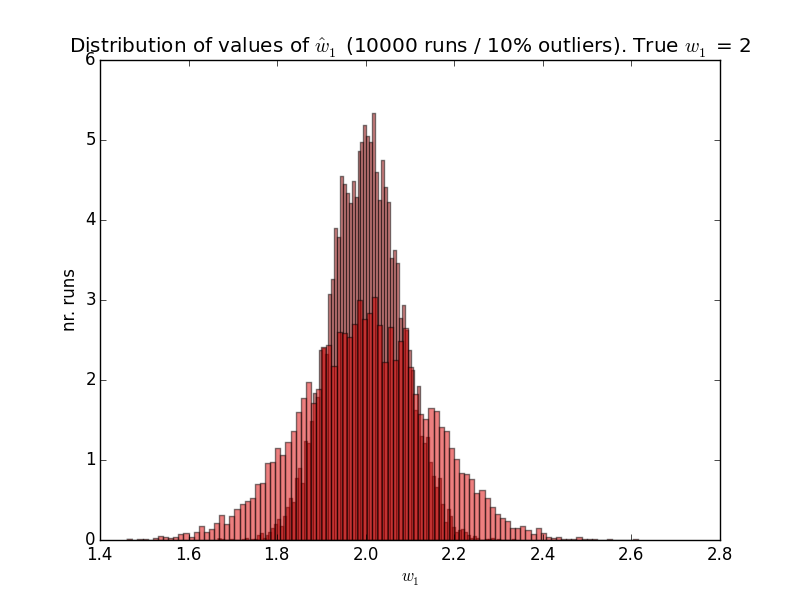
\includegraphics[width=1.0\linewidth]{chapter_lad/ols_w1_with_and_without_outliers.png}
\end{minipage}
  \label{fig.ols_estimates_no_outliers}
  \caption{The distribution of the estimates of the values of $w_0$ and $w_1$ for 10000 runs of OLS estimation, for two reference dataset of 500 point, one with no outliers (darker) and one with outliers (lighter)}
\end{figure}


The reason is that the squared loss will weight desproportionally the larger errors. So, if there is are a few points that 



\begin{figure}
\centering
\begin{minipage}{.5\textwidth}
  \centering
  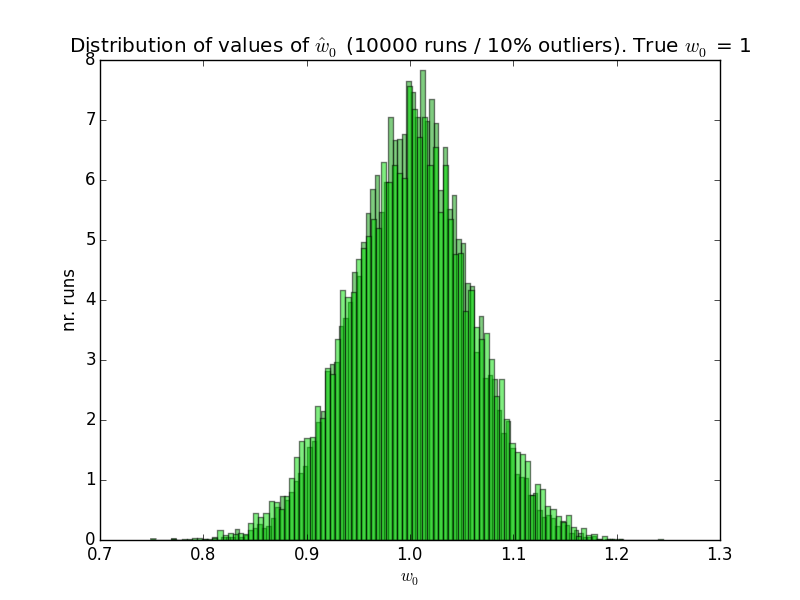
\includegraphics[width=1.0\linewidth]{chapter_lad/lad_w0_with_and_without_outliers.png}
\end{minipage}%
\begin{minipage}{.5\textwidth}
  \centering
  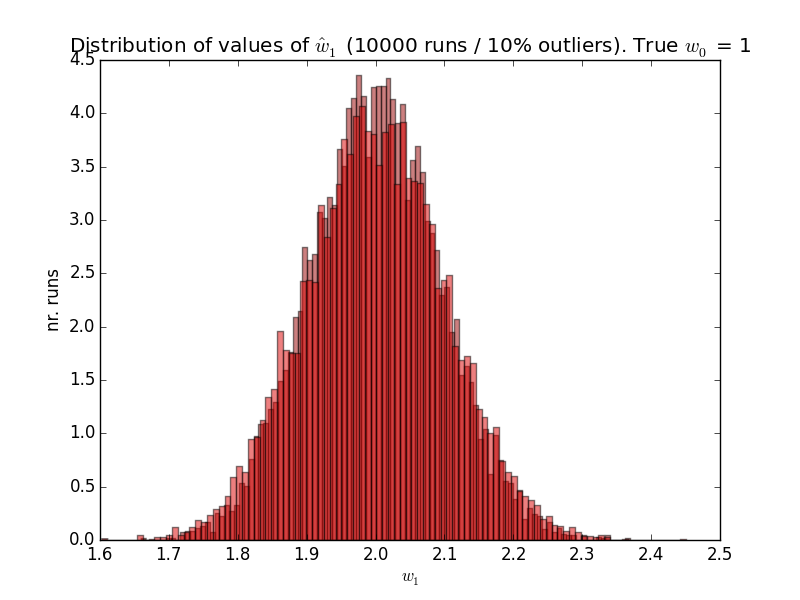
\includegraphics[width=1.0\linewidth]{chapter_lad/lad_w1_with_and_without_outliers.png}
\end{minipage}
  \label{fig.ols_estimates_no_outliers}
  \caption{The distribution of the estimates of the values of $w_0$ and $w_1$ for 10000 runs of LAD estimation, for two reference dataset of 500 point, one with no outliers (darker) and one with outliers (lighter)}
\end{figure}

